% Chapter 1

\chapter{Introduction} % Main chapter title

\label{Chapter1:introduction} % For referencing the chapter elsewhere, use \ref{Chapter1} 

%----------------------------------------------------------------------------------------
%1 page: Why you do this topic? Relevancy. What's the problem?
%1-2 page(s): What are you doing?
%1 page: Hence, this thesis tries to answer the following research question(s):
%total 4
%----------------------------------------------------------------------------------------

% Define some commands to keep the formatting separated from the content 
\newcommand{\keyword}[1]{\textbf{#1}}
\newcommand{\tabhead}[1]{\textbf{#1}}
\newcommand{\code}[1]{\texttt{#1}}
\newcommand{\file}[1]{\texttt{\bfseries#1}}
\newcommand{\option}[1]{\texttt{\itshape#1}}

%----------------------------------------------------------------------------------------


%1 page: Why you do this topic? Relevancy. What's the problem?
%----------------------------------------------------------------------------------------

Scene understanding is long existing and an interesting area for computer vision. Most of this is highly influenced by the binocular stereopsis of human visual three dimensional (3D) perception. Understanding the structural dependencies is one of the important task for 3D scene understanding and for its reconstruction, which is basically recovering the range and orientation of the surface and object to mimic the humans visual behaviour \cite{barnard1982computational}. This creates multiple opportunities for various multimedia computing applications.Most application requires only the oblique projection of 3D data into two dimensional (2D) plane such as 3D displays, movies, games or structural building representation. But in contrast there are also applications where these 3D depth information could be very important. Applications like augmented and virtual reality for immerse entertainment experience, pose estimation, object tracking, human activity estimation for robotics or autonomous driving systems etc., having a third dimension data which is depth could be vital. This shows the importance of having 3D depth information for these area of applications. \\

As a solution there are many techniques used to derive depth information. Most popular approaches can be categorized into three groups. First, dual camera method \cite{li2009dual} second,  dual pixel method \cite{martinello2015dual, choi2017all} and  third sensors based methods \cite{salvi2004pattern}. In extension various methods of estimating depth from focus \cite{grossmann1987depth}, stereo vision \cite{bulthoff1988integration}, and depth from motion \cite{ullman1979interpretation} where also applied. We will discuss more in detail in section \ref{Chapter3:RelatedWork_EarlyApproach}. In this study we mainly focus on sensor based methods, in which there are already some affordable sensing based-technologies for different application were developed. These types of sensors are called structure-light-system (SLS) \cite{salvi2004pattern}, which is based on the projection of structured light \cite{zhang2012microsoft}. Some of the examples for SLS depth sensors are Kinect v1 by Microsoft , Structure Sensor by Occipital, BlasterX Senz3D by Intel Realsense, Leap Motion Sensors by Leap Motion \cite{marin2014hand} and more are available \cite{mal2018sparse}. These devices have proven to have great impact in these areas but they come with a trade off with ease of use at consumer application end and we will discuss more about different SLS depth sensor in the following section \ref{Chapter4:Dataset}. Our study has the focus on depth estimation method based on SLSs, specifically Structure Sensor\footnote{https://structure.io/} by Occipital in the entire work.\\

Meanwhile as we know there is a remarkable interest grown in brain style computation and Artificial Neural Network (ANNs) is one of its derivative. ANNs have shown great versatility in the field of detection, classification and prediction. ANNs are used for many applications ranging from image processing \cite{guyon1991applications} , audio signal analysis \cite{bourlard1993continuous}, medical \cite{baxt1990use}, business science \cite{widrow1994neural}, music \cite{nadar2019towards} and many more \cite{zhang2000neural}. It  need a careful processing and considerable domain knowledge for representing a raw data into acceptable form for feature learning process. Another import aspect that comes with such brain style computation is hardware limitations towards computational complexity. But in recent days there are significant improvement in the heterogeneous computation \cite{mittal2015survey}. But often times these development always comes with a difficult trade off choices which has to be made between cost, power consumption and good throughput platforms for ANN's developments and implementations \cite{mittal2019survey}. \\




\section{Motivation}
\begin{figure}[!b]
    \centering
    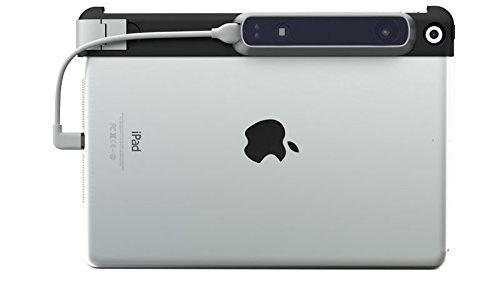
\includegraphics[width = 12cm]{Figures/ipad.jpg}
    \caption{Structural SensorImage Scource: Amazon.com}
    \label{fig:Structural_Sensor}
\end{figure}{}

Having a rich scene understanding of indoor spaces can answer various problems related to robotics, human activity recognition etc. also in some of the immersive experience and interactive technologies like  virtual reality and augmented reality applications where positional tracking and scene knowledge is crucial.

One of our interest is to achieve a good scene understanding related to depth information for indoor environment. This might open the doors of opportunities for various multimedia applications where depth information could be very crucial. One such example is \textit{IKEA Place} - an application developed by Apple in partnership with Ikea. \textit{IKEA Place} helps you to measure and place a 3D model of furniture from the Ikea catalog \cite{lehnert2017neue}. The furniture is represented as a 3D model in camera-enabled mobile device in this application \textit{IKEA Place}. One can walk around, bringing the piece of furniture in your camera-enabled mobile device and look at it from all sides and see where it can fit in your new house. This is one of the application where depth information could be used. To look at this concept of \textit{IKEA Place} in different perspective, we can recreate the entire indoor space as a 3D model and one can modify each element of their living or working spaces in a personalized fashion. This is one of the example idea where the depth information and 3D reconstruction of a indoor environment concepts can be used, this can be scaled up for various other application as well. Hence the applications of 3D reconstruction of indoor environment can have a wide range of usability. Similarly to the above mentioned application of 3D reconstruction, consumer level usability is also our main focus when applying depth estimation methods.  This is because, even though various efficient methods has been proposed based on the projection of structured light (as discussed in introduction and will be discussed in section \ref{Chapter3:RelatedWork} in detail) are available, the application at the consumer level might be challenging with respect to configuration, portability and background knowledge for usability. As we are discussing at consumer level usability, one of the areas we can look into is portable mobile device cameras. Nowadays, vast majority of cameras distributed in the market are embedded in mobile devices. These cameras have constraints on physical size, mechanical parts and processing capacity \cite{lee2007constraints}. Photographs from portable mobile devices are found to be a new approach for 3D reconstruction besides various traditional sensor based methods \cite{micheletti2015investigating, adan20113d}. In other words 3D image reconstruction from 2D images is our focus and motivation to find a solution in this area. In this context, in our project we utilized Structure Sensor manufactured by company called Occipital which is as SLS for portable mobile devices like Apple IPads as shown in figure \ref{fig:Structural_Sensor}. This comes with an additional hardware installation. Also there have been some efforts made towards low cost and efficient indoor 3D reconstruction using images collected with portable mobile devices or consumer level cameras \cite{ding2019low} but often time these accuracy or quality of these methods always have a trade off with resources like hardware (using SLS, camera quality) or computational efficiency.

In summary, as we understand the importance of depth estimation and its possibilities of remarkable applications in various areas, our motivation in this work is 3D reconstruction of a scene from a given 2D RGB image information which will lead to made consumer level application. For this we also want to answer if we can use brain style computational Artificial Neural Network (ANN) methods because we believe that by implementing a software based method might reduce the complexity at users end but with a trade off of computational power. With the growth of computational power, we believe that it is very much plausible to implement ANN models to consumer level applications in near future.

\section{Topic Description}
\label{Chapeter1:Topic_Description}
\begin{figure}[h]
    \centering
    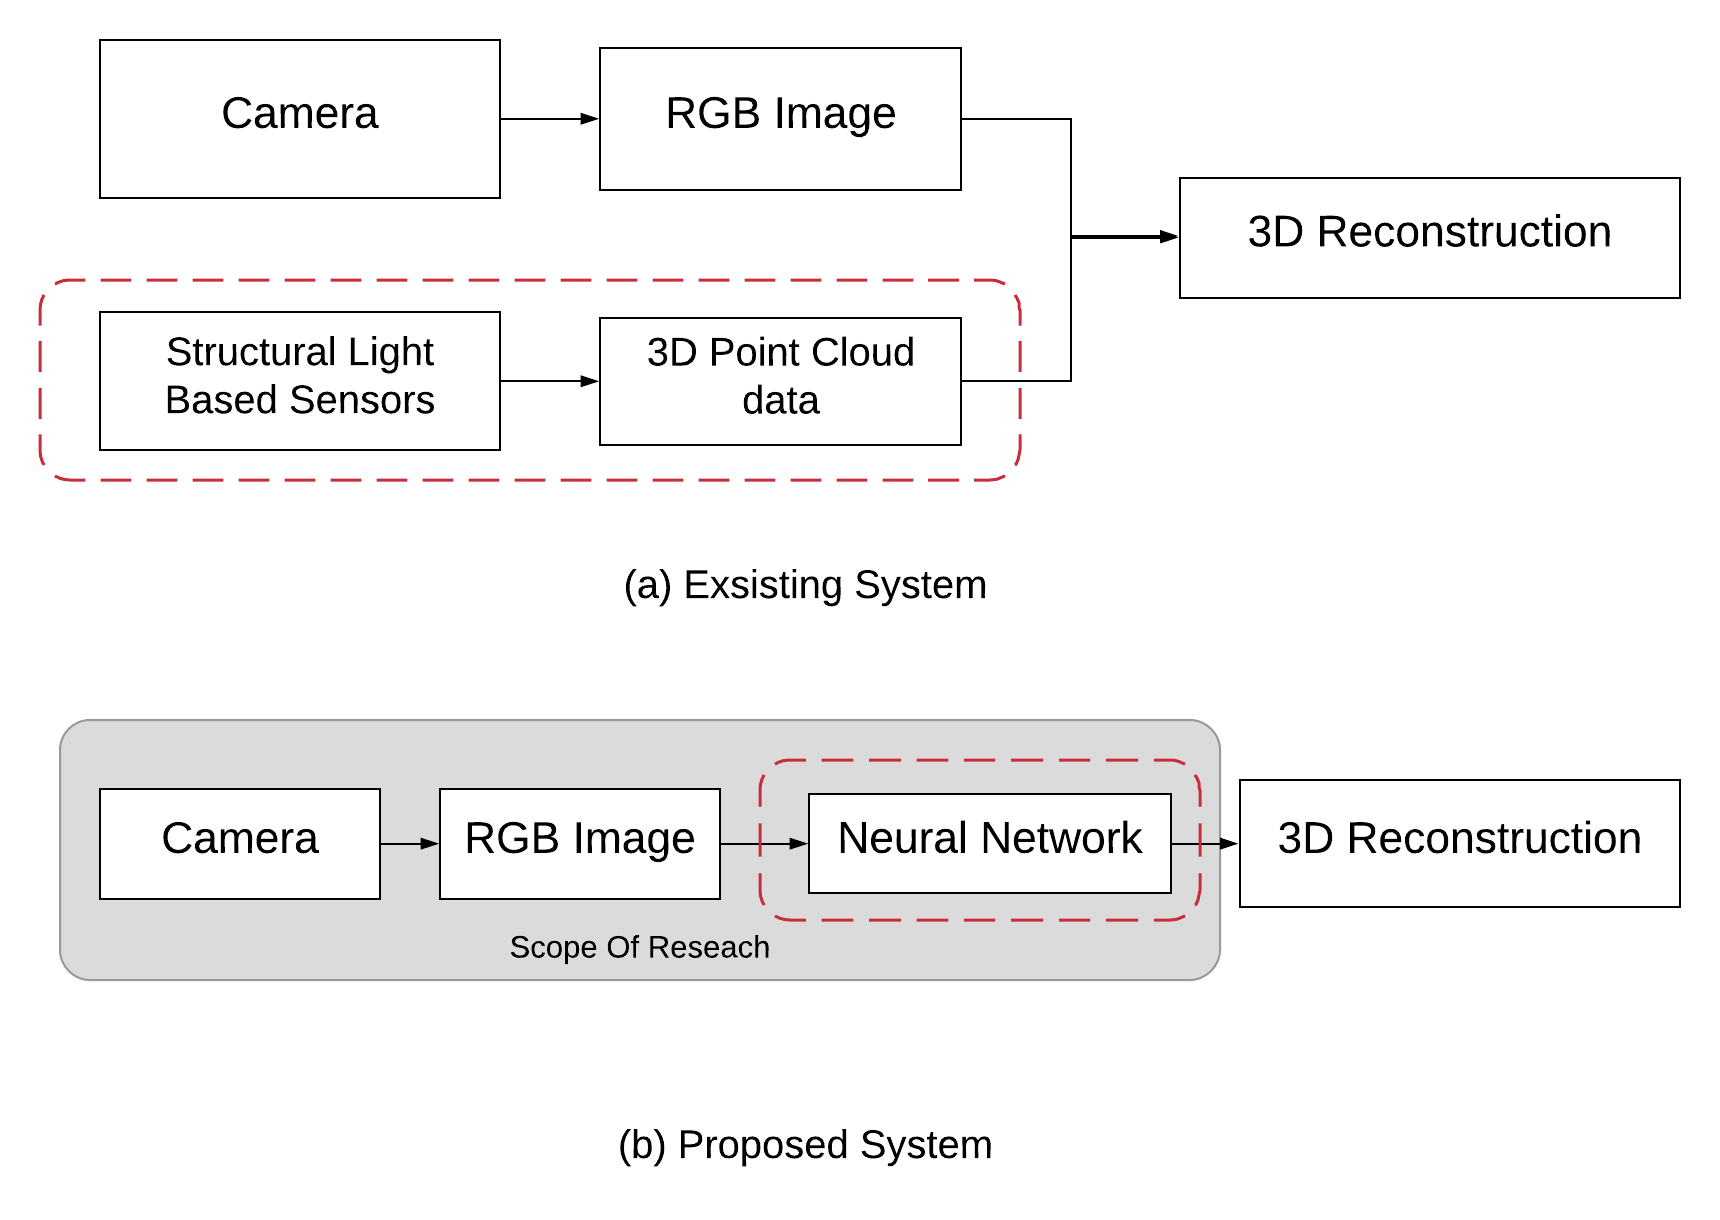
\includegraphics[width = 12cm]{Figures/idea.png}
    \caption{Topic Idea: The highlighted region in red box from existing system (a) is replaced by highlighted region in red box in proposed method (b)}
    \label{fig:Proposed_Model}
\end{figure}{}
%1-2 page(s): What are you doing?
This study proposes neural networks as an algorithm of depth estimation, more specifically using Convolutions Neural Networks(CNNs). The solution should define concise and accurate pixel for 3D reconstruction. Therefore, the goal is to achieve high accuracy in identifying the depth, especially boundaries of closer objects since the application is in indoor environment. Meanwhile, keeping the network operating speeds at a satisfying level, but the final implementation of this network will be on larger processing unit not in mobile device. This could be achieved by choosing a network architecture wisely with an attention to the details of the problem. Monocular depth estimation is based on ex-ploiting both local properties of texture, gradients, and color, as well as global geometric relations, like relative object placement, and perspective cues \cite{saxena2006learning}. Hence having a global structural understanding of image by Neural Network is very important and at the same time pixel level details for smaller object is also important in a scene. Often times the indoor environment could be more complex than outdoor because of several smaller objects in a scene. For example in office environment, there could be various physical objects on the table where as in outdoor environment having to deal with relatively larger object dimensions are more common.  

Aim of this project is to deliver a robust method and an architecture for depth image prediction replacing the sensor. As shown in figure \ref{fig:Proposed_Model} (a) Existing System for 3D reconstruction rely on hardware based implementation of a SLS which in our case is Structure Sensor integrated with Ipad as seen previously in Figure \ref{fig:Structural_Sensor}. This is done using Apple AR kit implementation which gives 2D RGB image from IPad and its depth information from the Structure Sensor and together are sent for further processing of 3D reconstruction. Thus our primary goal is to replace the existing system highlighted in red box as shown in Figure \ref{fig:Proposed_Model} (a) which consists of the structural light based sensors and the 3D point cloud data with a Neural Network as shown in the highlighted box in Figure \ref{fig:Proposed_Model}(b). We take advantage of Neural network as this has proven to give great results which we will see in details in section \ref{Chapter3:RelatedWork}.


Secondly, existing solutions to depth estimation from a single image usually rely on assumptions in which all the far field depth are mapped to a certain threshold which can result as a wall in 3D reconstruction from 2D. For example, the depth range of Kinet v2 sensor range from 0.5 meters (m) to 4.5m, which means that Kinet has a threshold that maps range above 4.5m to the maximum value of 4.5m that in turns results a wall. \cite{Silberman:ECCV12}. In practical implementation for 3D reconstruction its undesirable for us to have wall. Whereas the possibilities of the the output from SLB or Kinet sensors might give a inaccurate depth and most often times dead pixel - which is also called as holes for range above any threshold (for Kinet v2 is 4.5m) \cite{kinecttof}. Another very important reason for having holes is to get perfect reconstruction - ideally we can repaint the holes by changing the position of camera and not by any post processing methods which gives us better pixel level accuracy than in painting it, hence rather than approximation the values around holes, it is important for us to have information about these holes. In our work we are also interested to address this problem. We wanted the the network to learn these holes mimicking the SLS along with the relative depth of the scene for efficient regeneration of 3D scene. 

Thirdly, We were also interested to study about the effect of different camera and sensor properties in depth estimation mimicking the  Structure Sensor. This is because as we discussed earlier there are various types of SBL sensors avalable which has different properties. We will discuss in detail about these differences in following section \ref{Chapter4:Dataset}. Another reason for this study is because, most of the indoor scene depth estimations are based developed based on the dataset created by Kinet sensors, one such example is NYU\_v2 dataset \cite{silberman11indoor} which We will also discuss more in detail in related work section \ref{Chapter3:RelatedWork}. Thus Structure Sensor and Kinet sensor have different properties with respect to both sensors and cameras (which is used to map the relative color pixel) which brings us to a question how a Neural Network trained on different dataset influence the depth map suitable for images from IPad.  

These three problems gives us a clear direction to formulates some of the specific questions to be answered in this work which is described below. 


\section{Research questions and scientific contributions}
%1 page: Hence, this thesis tries to answer the following research question(s):

This work tries to address the following two questions:
\begin{itemize}
    \item RQ1: Can a Neural Network mimic SLS in predicting relative depth of a scene?
    \item RQ2: Can a Neural Network learn to regenerate the holes from a given depth information available from ?
    \item RQ3: Can a Neural Network learn Different Camera intrinsic and extrinsic parameters?  
\end{itemize}

In order to answer the three questions mentioned above, we propose a state-of-the-art approach using neural networks for this problem. Also generation of a new dataset is required to answer RQ2 and RQ3. This is because our goal is to achieve a model which replaces a specific SLS which is Structure Sensor and also most of the approach does not focus in retrieving the holes and existing dataset like Cornell Dataset \cite{3Dscene} , Washington Data V2 \cite{Washington}, Berkeley 3-D Object dataset (B3DO) \cite{Janoch:EECS-2012-85} etc. fail to provide with the holes except NYUv2 dataset with contains raw data information we will discuss more about the dataset in detain in section \ref{Chapter4:Dataset}. To give a justified reason for RQ3, we need to generate new dataset to have a common ground for comparison. 

Our three main contributions for this work are first, proposed a neural network model for depth map generation and compare with state of the art results. Secondly to deliver model which performs as good as Structure Sensor. Thirdly,  we created a new dataset based on Structural (SLB) Sensor.

Ultimately aim to achieve a similar working neural network model replacing Structural (SLB) sensor. This might reduce the complexity in users with a trade off of computational power. In the initial phase of this research our scope of study is to generate the 3D depth maps from neural networks after training on similar depth data. All the computation and evaluation were performed and tested with high processing unit which is described in details in Section \ref{Chapter5:HardwarSoftwareDetails}.


